\documentclass{ctuthesis}

\usepackage{tikz}
\usetikzlibrary{shapes.geometric, arrows.meta, automata}
\usepackage[sorting=none]{biblatex}
\addbibresource{bibliography.bib}
\usepackage{csquotes}
\usepackage{subcaption}

\newcommand{\bfc}[1]{\noindent{\color{ctublue}\textbf{#1}}\nopagebreak}
\newcommand{\CC}{{C\nolinebreak[4]\hspace{-.05em}\raisebox{.4ex}{\tiny\bf ++}}}

\ctusetup{
xdoctype = B,
xfaculty = F3,
mainlanguage = english,
titlelanguage = english,
title-english = {Autonomous road crossing with a mobile robot},
title-czech = {Autonomní přejezd silnice mobilním robotem},
specification-file = {zadani.pdf},
front-specification = {true},
keywords-english = {Autonomous robot operation, behavior trees, collision avoidance, collision detection, finite-state machines, road crossing, ROS},
keywords-czech = {Autonomní operace robota, detekce kolizí, konečné stavové automaty, přejíždění silnic, ROS, rozhodovací stromy, vyhýbání se kolizím},
department-english = {Department of Cybernetics},
author = {Jan Vlk},
fieldofstudy-english = {Cybernetics and Robotics},
fieldofstudy-czech = {Kybernetika a Robotika},
supervisor = {Mgr. Martin Pecka, Ph.D.},
supervisor-address = {Vision for Robotics and Autonomous Systems,\\ Resslova 9,\\ 12000 Praha 2},
month = 6,
year = 2023,
}
\ctuprocess
\begin{abstract-english}
    In this thesis, our task was to design, implement and evaluate an algorithm for the safe crossing of public roads with a middle-size mobile robot.\\
    The first part of this task is to conclude whether it is safe to cross the road in the robot's current location.  If it is, the second part of the task is developing a control algorithm to perform the movement needed to cross the road. Continuous monitoring of the traffic situation is necessary for the safety of the maneuver.\\
    We are also to provide evaluation metrics for determining the functionality and optimality of developed algorithms. The verification and evaluation of the developed algorithm will be conducted in simulation and a controlled real-world experiment.
    %In this thesis, it was our task to design, implement and evaluate an algorithm for crossing roads with a middle-size mobile robot. The first part of this task is to conclude whether it is safe to cross the road in the spot the robot is currently situated. If it is, the second part of the task is to perform the actual movement needed to cross the road.\\
    %We are to also provide evaluation metrics for determining the functionality and optimality of developed algorithms.
\end{abstract-english}
\begin{abstract-czech}
    V této práci je naším úkolem navrhnout, implementovat a vyhodnotit algoritmus pro bezpečný přejezd silnic s mobilním robotem střední velikosti.\\
    První část úkolu je zjistit, zda je bezpečné přejít silnici v místě, kde se robot právě nachází. Pokud ano, druhá část úkolu je navrhnout algoritmus pro řízení pohybu potřebného k přejetí silnice. Pro bezpečnost manévru je nutné provádět kontinuální monitorování dopravní situace.\\
    V neposlední řadě je třeba navrhnout metriku pro vyhodnocení funkčnosti a optimálnosti vyvinutých algoritmů. Verifikaci a vyhodnocení vyvinutého algoritmu provedeme v simulaci a v kontrolovaném experimentu v reálném světě.
    %V této práci je naším úkolem navrhnout, implementovat a vyhodnotit algoritmus pro přejezd silnic s mobilním robotem střední velikosti. První část úkolu je zjistit, zda je bezpečné přejít silnici v místě, kde se robot právě nachází. Pokud ano, druhá část úkolu je provést následné přejetí silnice.\\
    %Dále je třeba navrhnout metriku pro vyhodnocení funkčnosti a optimálnosti vyvinutých algoritmů.
\end{abstract-czech}
\begin{thanks}
    I would like to express my sincere gratitude to everyone who supported me throughout the completion of this bachelor's thesis. My most profound appreciation goes to my advisor, Martin Pecka, for his invaluable guidance, feedback and support throughout the research and development process.\\
    I am also grateful to my family and friends for their unwavering support and motivation. Their love and encouragement kept me motivated to finish this thesis and achieve this milestone.\\
    Finally, I want to acknowledge the faculty staff who generously shared their time for this research in its experimental phase. Their willingness to participate enabled me to conduct this study and make meaningful contributions to the field.\\
    Thank you all for your support and encouragement!
\end{thanks}
\begin{declaration}
    I declare that the presented work was developed independently and that I have listed all sources of information used within it in accordance with the methodical instructions for observing the ethical principles in the preparation of university theses.

    \medskip

    Prague, \today

    \vspace*{2cm}

    Prohlašuji, že jsem předloženou práci vypracoval samostatně a že jsem uvedl veškeré použité informační zdroje v souladu s Metodickým pokynem o dodržování etických principů při přípravě vysokoškolských závěrečných prací.

    \medskip

    Praha, {\selectlanguage{czech}\today}
\end{declaration}
\begin{document}
    \maketitle

    \chapter*{Introduction}
    In today's world, mobile robots are increasingly being utilized in a variety of applications. In many of these applications, the robots must cross roads to achieve their goals, making it essential to design an algorithm that enables the robot to cross the road safely.\\
    The algorithm should be able to determine whether the current place is suitable for crossing. The algorithm will accept contextual inputs such as vehicle velocity data, road type, number of lanes, and the presence of a pedestrian crossing with or without traffic lights. These data will be used to assess the current situation and determine whether it is safe to cross the road. If it is, it should facilitate the crossing itself. If the location is not suitable, the algorithm should provide a reason and suggest a more appropriate location nearby. The algorithm must also be designed to operate on different robots with various sensor configurations and road types without limitations.\\
    This thesis aims to provide a theoretical background to the problem and explore possible solutions. We will also present the hardware and software used for real-world and simulation experiments. We will discuss our chosen approach and its functionality and present the algorithms we developed and implemented. Finally, we will explain the results of our experiments and discuss their significance.\\
    Our work also depends on the output of other projects, such as vehicle detection and localization or path planning. We cannot rely on these projects to be completed or entirely functional. Therefore, we need a way to simulate and test our algorithm without them.\\
    In simulation experiments, we will inject data directly into our algorithm. For real-world experiments, we will try to use the outcomes of the projects mentioned earlier. However, we can inject data directly into our algorithm, provided the projects are not finished or functional.\\
    \newpage
    \section*{Used abbreviations}
        \begin{itemize}
            \item \textbf{AI} -- Artificial Intelligence
            \item \textbf{API} -- Application Programming Interface
            \item \textbf{BT} -- Behavior Tree
            \item \textbf{CRAS} -- Center for Robotics and Autonomous Systems
            \item \textbf{ENU} -- East-North-Up
            \item \textbf{FSM} -- Finite State Machine
            \item \textbf{GNSS} -- Global Navigation Satellite System
            \item \textbf{GPS} -- Global Positioning System
            \item \textbf{GUI} -- Graphical User Interface
            \item \textbf{HFSM} -- Hierarchical Finite State Machine
            \item \textbf{IMU} -- Inertial Measurement Unit
            \item \textbf{LiDAR} -- Laser imagining Detection and Ranging
            \item \textbf{NED} -- North-East-Down
            \item \textbf{NPC} -- Non-Player Character
            \item \textbf{OSM} -- Open Street Map
            \item \textbf{REP} -- ROS Enhancement Proposals
            \item \textbf{RL} -- Reinforcement Learning
            \item \textbf{ROS} -- Robot Operating System
            \item \textbf{TPI} -- Terrain Profile Index
            \item \textbf{UTM} -- Universal Transverse Mercator
            \item \textbf{WGS84} -- World Geodetic System 1984
            \item \textbf{ZABAGED} -- Základní báze geografických dat (Basic database of geographic data)
        \end{itemize}
    

    \chapter{Theoretical background}
        \section{Behavior trees}
    A behavior tree (BT) is a way to structure algorithms -- the switching between individual tasks in an autonomous agent. It was created to express behavior patterns for NPCs (non-player characters) in computer games. Since then, it has found many more applications, and nowadays, it is also widely used in robotics and AI applications.\\
    BTs, as the name suggests, are tree-like structures where each node represents an action, a condition, a control, or a decorator node. Action and control nodes are leaves of the tree structure. Control nodes are used to control and modify the flow of the tree. Examples of these nodes are \texttt{Sequence}, \texttt{fallback}, or \texttt{repeat}. Decorator nodes are used to modify the return values, thus modifying the behavior of its children. Examples of these nodes are \texttt{force-success}, \texttt{force-failure}, or \texttt{inverter}.\\
    The execution of a BT commences at the root node and then progressively traverses the tree structure in a depth-first fashion ticking its nodes. The nodes' ticking, also known as polling, is periodically repeated. Each node, once ticked, begins its execution process, and once finished, it returns a status. This status can be either \texttt{SUCCESS}, \texttt{FAILURE}, or \texttt{RUNNING}. The action and control nodes are responsible for determining and returning these states. The control nodes alter the tree's flow and tick handling based on its children's return states. Decorator nodes modify the return states of their children. The return states of some nodes are shown in table \ref{tab:returns}.
    \begin{table}[H]
        \centering
        \begin{tabular}{|l|l|l|l|}
            \hline
            Node type & \texttt{SUCCESS} & \texttt{FAILURE} & \texttt{RUNNING} \\
            \hline\hline
            \texttt{Action} & Action succeeds & Unable to complete & During completion \\
            \hline
            \texttt{Condition} & Condition is true & Condition is false & \emph{NA} \\
            \hline
            \texttt{Sequence} & All children succeed & One child fails & One child running \\
            \hline
            \texttt{Fallback} & One child succeeds & All children fail & One child running \\
            \hline
            \texttt{Parallel} & $N$ children succeed & $<N$ children succeed & Children running \\
            \hline
            \texttt{Repeat} & Child succeeds & Child fails $x$ times & Child running \\
            \hline
        \end{tabular}
        \caption{Return states of some nodes.}
        \label{tab:returns}
    \end{table}

    \noindent The first chapter in \cite{BT_intro} provides a more thorough explanation of the behavior trees.

    \subsection{Commonly used nodes}
        Here we will present the most commonly used nodes and their functionality.\\\\
        \textbf{Sequence} -- Control node that ticks its children one at a time in a predefined order. If one of the children were to return \texttt{FAILURE}, the ticking of other children is stopped, and the \texttt{Sequence} node returns \texttt{FAILURE}. The same happens if one of the children returns \texttt{RUNNING}. If all children return \texttt{SUCCESS} the \texttt{sequence} node returns \texttt{SUCCESS}.\\\\
        \textbf{Fallback} -- Also known as \texttt{Selector} is a control node that ticks its children one at a time in a predefined order. If one of the children were to return \texttt{SUCCESS}, the ticking of other children is stopped, and the \texttt{fallback} node returns \texttt{SUCCESS}. The same happens if one of the children returns \texttt{RUNNING}. If all children return \texttt{FAILURE} the \texttt{fallback} node returns \texttt{FAILURE}.\\\\
        \textbf{Parallel} -- Control node that allows multiple actions to run concurrently. It returns \texttt{SUCCESS} if $N$ or more children return \texttt{SUCCESS} and \texttt{FAILURE} if less than $N$ children return \texttt{SUCCESS}. If all children return \texttt{RUNNING} the \texttt{parallel} node returns \texttt{RUNNING}.\\\\
        \textbf{Repeat} -- Control node that ticks its child a specified number of times or until the child returns \texttt{SUCCESS}, whichever comes first. If the child returns \texttt{RUNNING}, the \texttt{repeat} node returns \texttt{RUNNING}. If the child does not return \texttt{SUCCESS} before the number of repetition is reached the \texttt{repeat} node returns \texttt{FAILURE}.\\\\
        \textbf{Inverter} -- Decorator node that inverts the return state of its child. If the child returns \texttt{SUCCESS}, the \texttt{inverter} node returns \texttt{FAILURE} and vice versa. If the child returns \texttt{RUNNING} the \texttt{inverter} node returns \texttt{RUNNING}.\\\\
        \textbf{Force-success} -- Decorator node that returns \texttt{SUCCESS} regardless of the return state of its child.\\\\
        \textbf{Force-failure} -- Decorator node that returns \texttt{FAILURE} regardless of the return state of its child.

    \subsection{Graphical representation of BTs}
        We will represent the BTs in this work in the following way. Action nodes will be rectangular with the name of the action written inside. Control nodes will be elliptical with the name of the condition written inside. Control and decorator nodes will be rectangular with a corresponding symbol inside. The symbols are shown in table \ref{tab:symbols}.\\
        If the BT has a sub-tree in its structure, we will represent it as a diamond-shaped node with the sub-tree's name written inside.
        \begin{table}[H]
            \centering
            \begin{tabular}{|l|l|c|}
                \hline
                \textbf{Node type} & \textbf{Description} & \textbf{Symbol} \\
                \hline\hline
                \texttt{Root} & The root of the tree & $Root$ \\
                \hline
                \texttt{Sequence} & Ticks its children if the return is \texttt{SUCCESS} & $\to$ \\
                \hline
                \texttt{Fallback} & Ticks its children if the return is \texttt{FAILURE} & $?$ \\
                \hline
                \texttt{Parallel} & Allows multiple actions to run concurrently & $\rightrightarrows$ \\
                \hline
                \texttt{Repeat} & Repeats the child node $x$ times & $\circ(x)$ \\
                \hline
                \texttt{ForceSuccess} & Allways returns \texttt{SUCCESS} & $\checkmark$ \\
                \hline
                \texttt{ForceFailure} & Allways returns \texttt{FAILURE} & $\times$ \\
                \hline
                \texttt{Inverter} & Inverts the return value of its child & $\neq$ \\
                \hline
            \end{tabular}
            \caption{Symbols used for control and decorator nodes in BTs.}
            \label{tab:symbols}
        \end{table}
    
    \subsection{BT example}
        We will present a simple example demonstrating the BTs structure and design principles.\\
        The example BT is shown in figure \ref{fig:example_tree}. This BT was created in the algorithm design's beginning phase, and its modified version will be presented later as it is used in the final implementation. The goal of this sub-tree was to position the robot so that it would cross the road as fast as possible, meaning we want the robot to stand perpendicular to the road.
        \begin{figure}[H]
            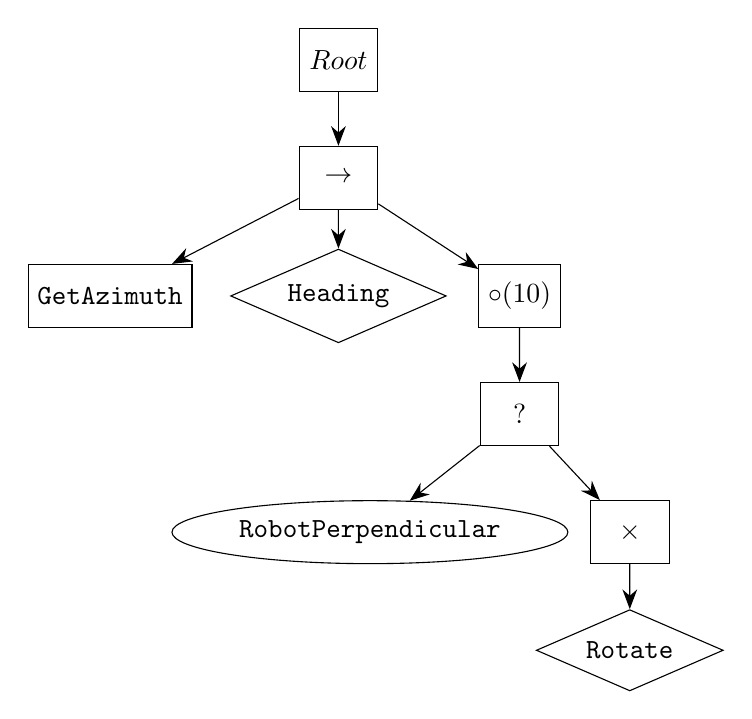
\begin{tikzpicture}[sibling distance=28mm, minimum width=1cm, minimum height=0.8cm]
                \node [draw] {$Root$}
                    child {node [draw] {$\to$} edge from parent [-{Stealth[length=2.5mm]}]
                    child {node [draw, xshift=0-.1cm] {\texttt{GetAzimuth}}}
                    child {node [diamond, draw, aspect=2.3] {\texttt{Heading}}}
                    child {node [draw, xshift=0-.5cm] {$\circ(10)$}
                    child {node [draw] {?}
                    child {node [ellipse, draw, xshift=0-0.5cm] {\texttt{RobotPerpendicular}}}
                    child {node [draw] {$\times$}
                    child {node [diamond, draw, aspect=2.3] {\texttt{Rotate}}}}}}};
            \end{tikzpicture}
            \caption{BT example.}
            \label{fig:example_tree}
        \end{figure}
        We start in the root node and continue straight to the \texttt{Sequence} node. From there, we go to the action node \texttt{GetAzimuth}, which gives us the current heading of the robot. If the execution of the \texttt{GetAzimuth} node is successful, we continue to the \texttt{Heading} sub-tree node. This sub-tree aims to calculate the heading the robot needs to achieve in order to be perpendicular. If the execution of the sub-tree is successful, we continue to the \texttt{Repeat} node. This node will repeat its children ten times (or less if success is achieved sooner). The first child we will tick is a \texttt{Fallback} node, with its first child being a condition node \texttt{RobotPerpendicular}. The condition node return value states whether or not the robot is already perpendicular to the road, we mean to cross. If we are not yet perpendicular, we continue. The next node we tick is a \texttt{Force-Failure} node with a sub-tree node as its child. The sub-tree is responsible for rotating the robot to the desired heading.

    \subsection{Other used BT nodes}
        Here we will present other BT nodes. These nodes are an expansion of the common ones and are implementation specific.\\\\
        \textbf{SequenceStar} ($\to^{*}$) -- Also know as \texttt{SequenceWithMemory}, a control node that functions in the same way as \texttt{Sequence}. The only difference is that this node does not repeat children that returned \texttt{SUCCESS} until all children have. Meaning until the \texttt{SequenceStar} node returns \texttt{SUCCESS}, it will tick only the children that have not succeeded yet.\\\\
        \textbf{ReturnSuccess} -- A leaf node that returns \texttt{SUCCESS} once ticked. We will represent this node as an ellipse with a checkmark character ($\checkmark$) inside.\\\\
        \textbf{ReturnFailure} -- A leaf node that returns \texttt{FAILURE} once ticked. We will represent this node as an ellipse with a cross character ($\times$) inside.

    \subsection{Common BT structures}
        Common programming principles can explain some BT structures. We will present a few of these structures that we have used in our BT structure.\\\\
        \bfc{If-else}\\
            The \texttt{if-else} structure starts with a \texttt{Fallback} node, and the first child a \texttt{Sequence} node with its first child a condition node and second child an action node, ticked if the condition is true. The second child of the \texttt{Fallback} node is also an action node that is performed if the condition is false.\\
            The structure is shown in figure \ref{fig:if-else}.\\\\
        \bfc{Condition-action}\\
            We could also name this structure as \texttt{if not}.\\
            The \texttt{condition-action} structure starts with a \texttt{Fallback} node. Its first child is a condition node, and its second is an action node. The idea behind this structure is to check if an action has been performed, and if it has not, we want to perform it.\\
            The structure is shown in figure \ref{fig:cond-action}.\\\\
        \begin{figure}[ht]
            \begin{subfigure}{0.49\textwidth}
                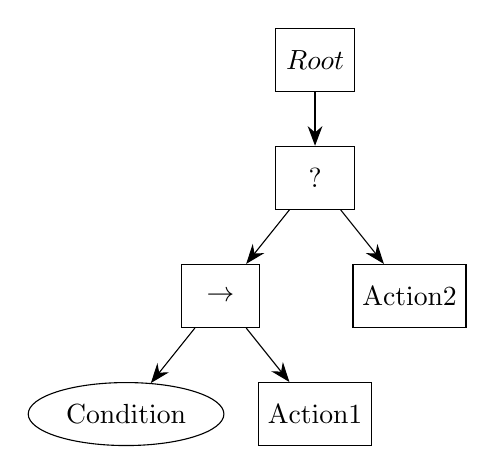
\begin{tikzpicture}[sibling distance=24mm, minimum width=1cm, minimum height=0.8cm]
                    \node [draw] {$Root$}
                        child {node [draw] {?} edge from parent [-{Stealth[length=2.5mm]}]
                        child {node [draw] {$\to$}
                        child {node [ellipse, draw] {Condition}}
                        child {node [draw] {Action1}}}
                        child {node [draw] {Action2}}};
                \end{tikzpicture}
                \caption{The \texttt{if-else} structure.}
                \label{fig:if-else}
            \end{subfigure}
            \begin{subfigure}{0.49\textwidth}
                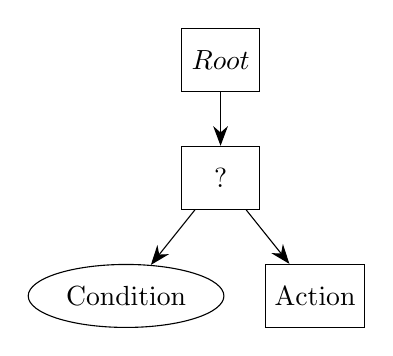
\begin{tikzpicture}[sibling distance=24mm, minimum width=1cm, minimum height=0.8cm]
                    \node [draw] {$Root$}
                        child {node [draw] {?} edge from parent [-{Stealth[length=2.5mm]}]
                        child {node [ellipse, draw] {Condition}}
                        child {node [draw] {Action}}};
                \end{tikzpicture}
                \caption{The \texttt{condition-action} structure.}
                \label{fig:cond-action}
            \end{subfigure}
            \caption{The common structures used in the creation of BTs.}
        \end{figure}

        \section{Finite-state machines}
    Finite-state machines (FSM) are a mathematical model of computation. They are used to model the behavior of a system in a finite number of pre-defined states. The system can be in only one state at a time. In each state, a computation or an action is performed. The change of a state is possible only via predetermined transitions triggered by a condition.\\
    FSMs are a common method of describing and solving high-level sequential control problems. They are used in many fields, such as robotics, computer science, electrical engineering, etc.\\
    FSM offers a very effective method in the implementation of complex robot behavior in comparison to monolithic programming.\cite{FSM_safety} Moreover, the learning curve for using FSM is minor; it is quite likely the reader already knows about FSMs from math or logic courses. Secondly, the integration itself is almost painless, especially when one takes the FSM into account from early stages of the design.\cite{FSM_intro}\\
    However, the FSMs are unsuitable for large and complex systems as they tend to become unmanageable and difficult to extend and reuse. This becomes more evident for a fully reactive system, where each state must be able to transition to any other state. Such a condition imposes the FSM to become a fully connected graph ($\mathcal{O}(n^2)$). Maintaining and modifying such a graph is quite a labor-intensive and error-prone task.\\
    FSMs are also unsuitable for systems requiring a high degree of autonomy. The FSMs are not able to learn and adapt to the changing environment.\\
    The formal definition of a FSM and several examples can be found in \cite{FSM_intro}.

    \subsection{FSM example}
        Here we will show the FSM for the example BT (figure \ref{fig:example_tree}) from the previous section.
        \begin{figure}[H]
            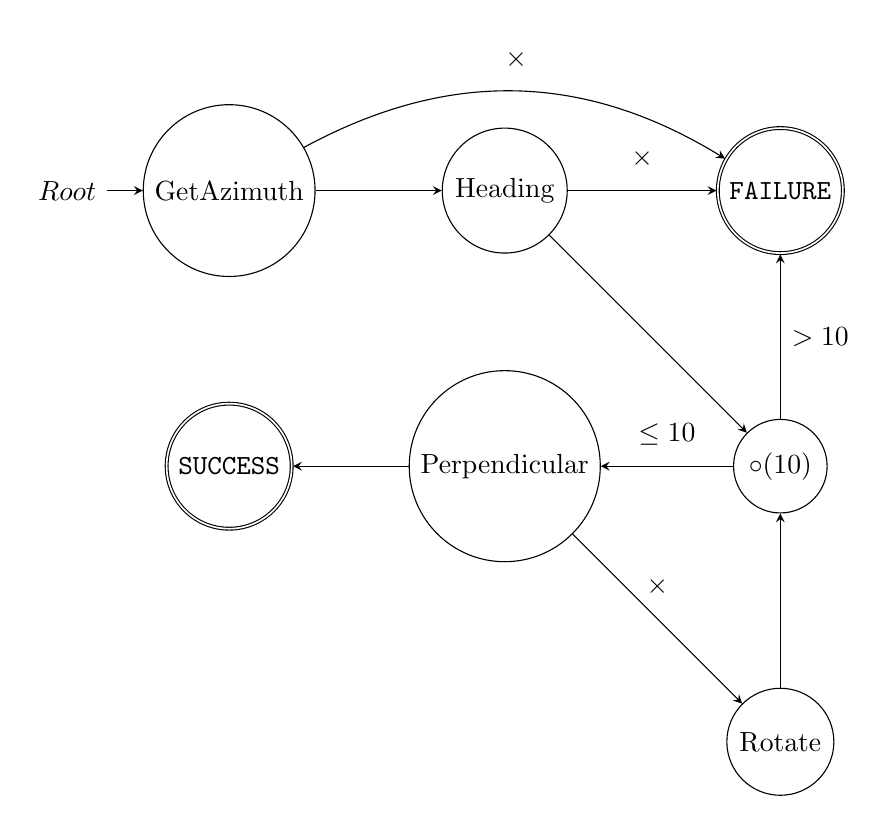
\begin{tikzpicture}[node distance=3.5cm, minimum width=1cm, minimum height=0.8cm, ->, >=stealth, initial text=$Root$]
                \node[state, initial] (azimuth) {GetAzimuth};
                \node[state, right of=azimuth] (heading) {Heading};
                \node[state, accepting, right of=heading] (failure) {\texttt{FAILURE}};
                \node[state, below of=failure] (repeat) {$\circ(10)$};
                \node[state, left of=repeat] (perpendicular) {Perpendicular};
                \node[state, below of=repeat] (rotate) {Rotate};
                \node[state, accepting, left of=perpendicular] (success) {\texttt{SUCCESS}};
                \draw   (azimuth) edge[above] node{$\checkmark$} (heading)
                        (azimuth) edge[above, bend left] node{$\times$} (failure)
                        (heading) edge[left] node{$\checkmark$} (repeat)
                        (heading) edge[above] node{$\times$} (failure)
                        (repeat) edge[above] node{$\leq10$} (perpendicular)
                        (repeat) edge[right] node{$>10$} (failure)
                        (perpendicular) edge[above] node{$\checkmark$} (success)
                        (perpendicular) edge[above] node{$\times$} (rotate)
                        (rotate) edge (repeat);
            \end{tikzpicture}
            \caption{FSM for the example BT.}
            \label{fig:example_fsm}
        \end{figure}
        This is not a typical representation of a FSM. It is a one to one rewrite of the BT example. If we were to develop the algorithm using FSMs, the FSM would look different. BTs and FSMs require different mindsets and design principles and while they may be rewritten from one to the other, it usually results in a nonoptimal structure.

\section{Hierarchical FSMs}
    Hierarchical state machines (HFSM), also known as statecharts, were developed to alleviate the cumbersome transition duplication required in large FSMs and add structure to aid comprehension of complex systems. It clusters states into a group (named superstate) where all the underlying internal states (substates) implicitly share the same superstate.\cite{BT_driving}\\
    While the HFSM solves the problem of transition duplication, it does not solve the complexity problem. The HFSM is still a fully connected graph unsuitable for large and complex systems.
        \section{Comparison and chosen approach}
    We can use several design approaches to solve the task of crossing a street. We will briefly present them and state a few advantages and disadvantages of each one. We will mainly use the informations and insights from \cite{BT_intro}.\\\\
    \bfc{Monolithic approach}\\
        We can use a monolithic approach, where we write a single program that will handle all the tasks.\\
        This approach is the most straightforward and easiest to implement but is not very flexible. It would be complicated to modify or extend the abilities of our program to the point where we would be forced to rewrite it in its entirety. This approach also generates a design that is not easily readable, and it would be almost impossible to find and correct bugs and glitches.\\
        For all those reasons, the monolithic approach is unsuitable for anything other than elementary systems, and we will not use it for our solution.\\\\
    \bfc{FSM approach}\\
        The second approach is to use an FSM. More specifically, HFSM as it is an improvement over FSM and addresses a few of the FSM issues.\\
        The advantages of HFSMs are that the structure is intuitive and generally easy to understand. Being common in many parts of computer science and used for quite some time, they are also easy to implement. FSMs also offer good flexibility and maintainability for many problems.\\
        The main disadvantage of HFSMs is that the flexibility is limited to certain areas of use and systems with limited scale. It is impossible to add new states or transitions in complex systems easily.\\
        The scalability of FSMs is also a problem. With rising demands on agent AI complexity, game programmers found that the FSMs that they used scaled poorly and were difficult to extend, adapt and reuse.\cite{BT_survey}\\
        The FSM's poor scalability makes this approach unsuitable for our solution.\\\\
    \bfc{BT approach}\\
        The third approach is to design the algorithm in the form of a BT.\\
        The advantages of this approach are its modularity, reusability, reactivity, readability, and scalability. Modularity is closely linked with reusability. The design principles of BTs allow us to decompose the algorithm into sub-trees which may be implemented and tested separately. Decomposition also allows us to tackle large complex systems with relative ease. The BTs are reactive in the sense that they can react quickly and effectively to the changing environment. Even though they require a different design approach than FSMs, they provide a coherent and compact structure that is easy to understand and maintain.\\
        The main disadvantage of BTs is that they are not very common in the industry and are not as well known as FSMs. For this reason, the tools and libraries are not as numerous or mature as those available for FSMs. As mentioned earlier, they are different from FSMs and, as such, require a different approach to designing an optimal solution.\\\\
    \bfc{Chosen approach}\\
        The approach we have chosen to use in this thesis is the BT approach. We have chosen it for many reasons, mainly its scalability, readability, and maintainability of large complex systems. The BTs are also very flexible and can be easily extended and modified. The supervisor also suggested the use of the BT approach.
        \section{Mathematical aparatus}
    This thesis will use chapters from linear algebra, calculus, geometry, and probability theory.\\
    The used theory will be shown and briefly explained in sections where it is needed. We will not provide precise definitions or state used theorems as it is outside the scope of this work. However, a book, a paper, or an online document with the corresponding information will be provided should the reader require a more thorough explanation.\\

\section{Maps}
    We will use the maps from the OpenStreetMap (OSM) project\footnote{\url{https://www.openstreetmap.org}}. The maps will be used to determine the surroundings of the robot and whether the current position is suitable for crossing.\\
    OSM is a project that creates and distributes free geographic data. The data is created by the community of users and is available for anyone to use.\cite{OSMwiki}\\
    The map data are expressed either by a node, a way, or a relation. Node is a singular point in map, it could be a landmark, a corner of building or a spot on the road. Way is an object created from multiple nodes. It can be either closed or open. Closed ways may represent a park, building or a some other type of area. Open ways commonly represent roads, rivers, or other linear features. Relation is a collection of nodes, ways, or other relations. It is used to describe more complex objects, such as a bus line, a building complex etc.

    \chapter{Used hardware and software}
        \section{Software}
    All work in this thesis is aimed to work with Robot Operating System (ROS) \cite{ROS}. We will use ROS1 in version Noetic Ninjemys\footnote{\url{http://wiki.ros.org/noetic}}.\\\\
    \bfc{Programming languages}\\
        The majority of implementation work will be done in a \CC\ programming language. The version of \CC\ standard used is \CC14, as it is the default for ROS1.\\
        The \CC\ language was chosen for its speed and efficiency. It was also chosen for some of the libraries we need to use for our project.\\
        The second programming language we will use is Python in version 3.8. Python was chosen for its simplicity and ease of use, as well as for using our previous work in OSM data processing.\\\\
    \bfc{BT library}\\
        There are a few possibilities regarding the BT library we can use for our solution. As BTs are not very commonly used, the choice is more limited than if we use FSM. Another limiting factor we have is support or direct integration with ROS.\\
        We still have a few options, and we can even choose a programming language in which to implement the BT nodes. The two programming languages with the most library options are \CC\ and Python. This copies the ROS mentality, where these two languages are natively supported. Some possibilities are discussed here \cite{BT_FSM}.\\
        We have decided to use a \CC\ behaviortree-cpp-v3 library\footnote{\url{https://github.com/BehaviorTree/BehaviorTree.CPP}}. The choice was made for multiple reasons. This library was written with deployment in ROS in mind. It is regularly updated and maintained, making it the safe choice for us. It also comes with a documentation that will be helpful during the implementation process. There are two version of the documentation \cite{BT_docs} and \cite{BT_docs_new}. We will mainly use the newer one (the second mentioned), but we will cross reference it with the older one.\\
        Another benefit of this implementation is that it comes with a GUI application for creating BTs called Groot\footnote{\url{https://github.com/BehaviorTree/Groot}}. This application creates an \texttt{.xml} file with the BT structure we can import into our code later.\\\\
    \bfc{Libraries for OSM and work with geographical data}\\
        There are a lot of libraries to choose from when it comes to working with OSM data. These libraries are created for different programming languages and have different features.\\
        Even though the majority of our work was written in \CC, we were building on top of previous work of assigning costs to road segments in OSM data. This work was done during the 2022 summer as a part of the RobInGas project here at the CTU under the Center for Robotics and Autonomous Systems (CRAS\footnote{\url{https://robotics.fel.cvut.cz/cras}}) group.\\
        The work was done in Python, and the library used was the overpy library\footnote{\url{https://github.com/DinoTools/python-overpy}}. This library is used to access the OSM Overpass API and download the map data. The Overpass API (formerly known as OSM Server Side Scripting) is a read-only API that serves up custom-selected parts of the OSM map data. The difference between the main API is that the Overpass API is optimized for small to large consumers (up to roughly 10 million elements). Many services and applications use it as a database backend.\cite{Overpass}\\
        Other libraries used for work with the OSM data were shapely\cite{shapely}, numpy\cite{numpy} and utm\footnote{\url{https://github.com/Turbo87/utm}}. These libraries were used to classify and assign costs to individual road segments in the downloaded OSM data.\\
        In our work, we also need to convert the coordinates of the robot from the GPS coordinate system to the UTM coordinate system. The conversion is done using the GeographicLib library\cite{GeographicLib}.
        \section{Hardware for real-world experiments}
    \subsection{Robots}
        In this section, we will present the robots available for use in the real-world experiments. We have two robotic platforms available for us: Husky and Spot.\\\\
        \bfc{Husky}\\
        Husky is a medium all-terrain robot developed by Clearpath Robotics. It is a four-wheeled robot with a payload capacity of 75 kg. The weight of this robot without the payload is 50 kg, and its maximal speed is $1\:\si{\m\per\s}$. This robot is mainly used outside of urban areas. The photo of the Husky in the configuration we use is shown in figure \ref{fig:husky}.\\
        More information about the Husky platform is available at the Clearpath Robotics website\footnote{\url{https://clearpathrobotics.com/husky-unmanned-ground-vehicle-robot/}}.\\\\
        \bfc{Spot}\\
        The Spot is a medium all-terrain robot developed by Boston Dynamics. It is a four-legged robot with a payload capacity of 14 kg. The weight of this robot without the payload is 33 kg, and its maximal speed is $1.6\:\si{\m\per\s}$. This robot is designed to be mainly used in urban and industrial areas. The photo of the Spot robot with our payload is shown in figure \ref{fig:spot}.\\
        More information is available at the Boston Dynamics website\footnote{\url{https://www.bostondynamics.com/sites/default/files/inline-files/spot-specifications.pdf}}.

        \begin{figure}[H]
            \centering
            \begin{subfigure}[b]{0.495\textwidth}
                \centering
                \includegraphics[width=\textwidth]{images/husky.jpg}
                \caption{The Husky robot configuration.}
                \label{fig:husky}
            \end{subfigure}
            \begin{subfigure}[b]{0.495\textwidth}
                \centering
                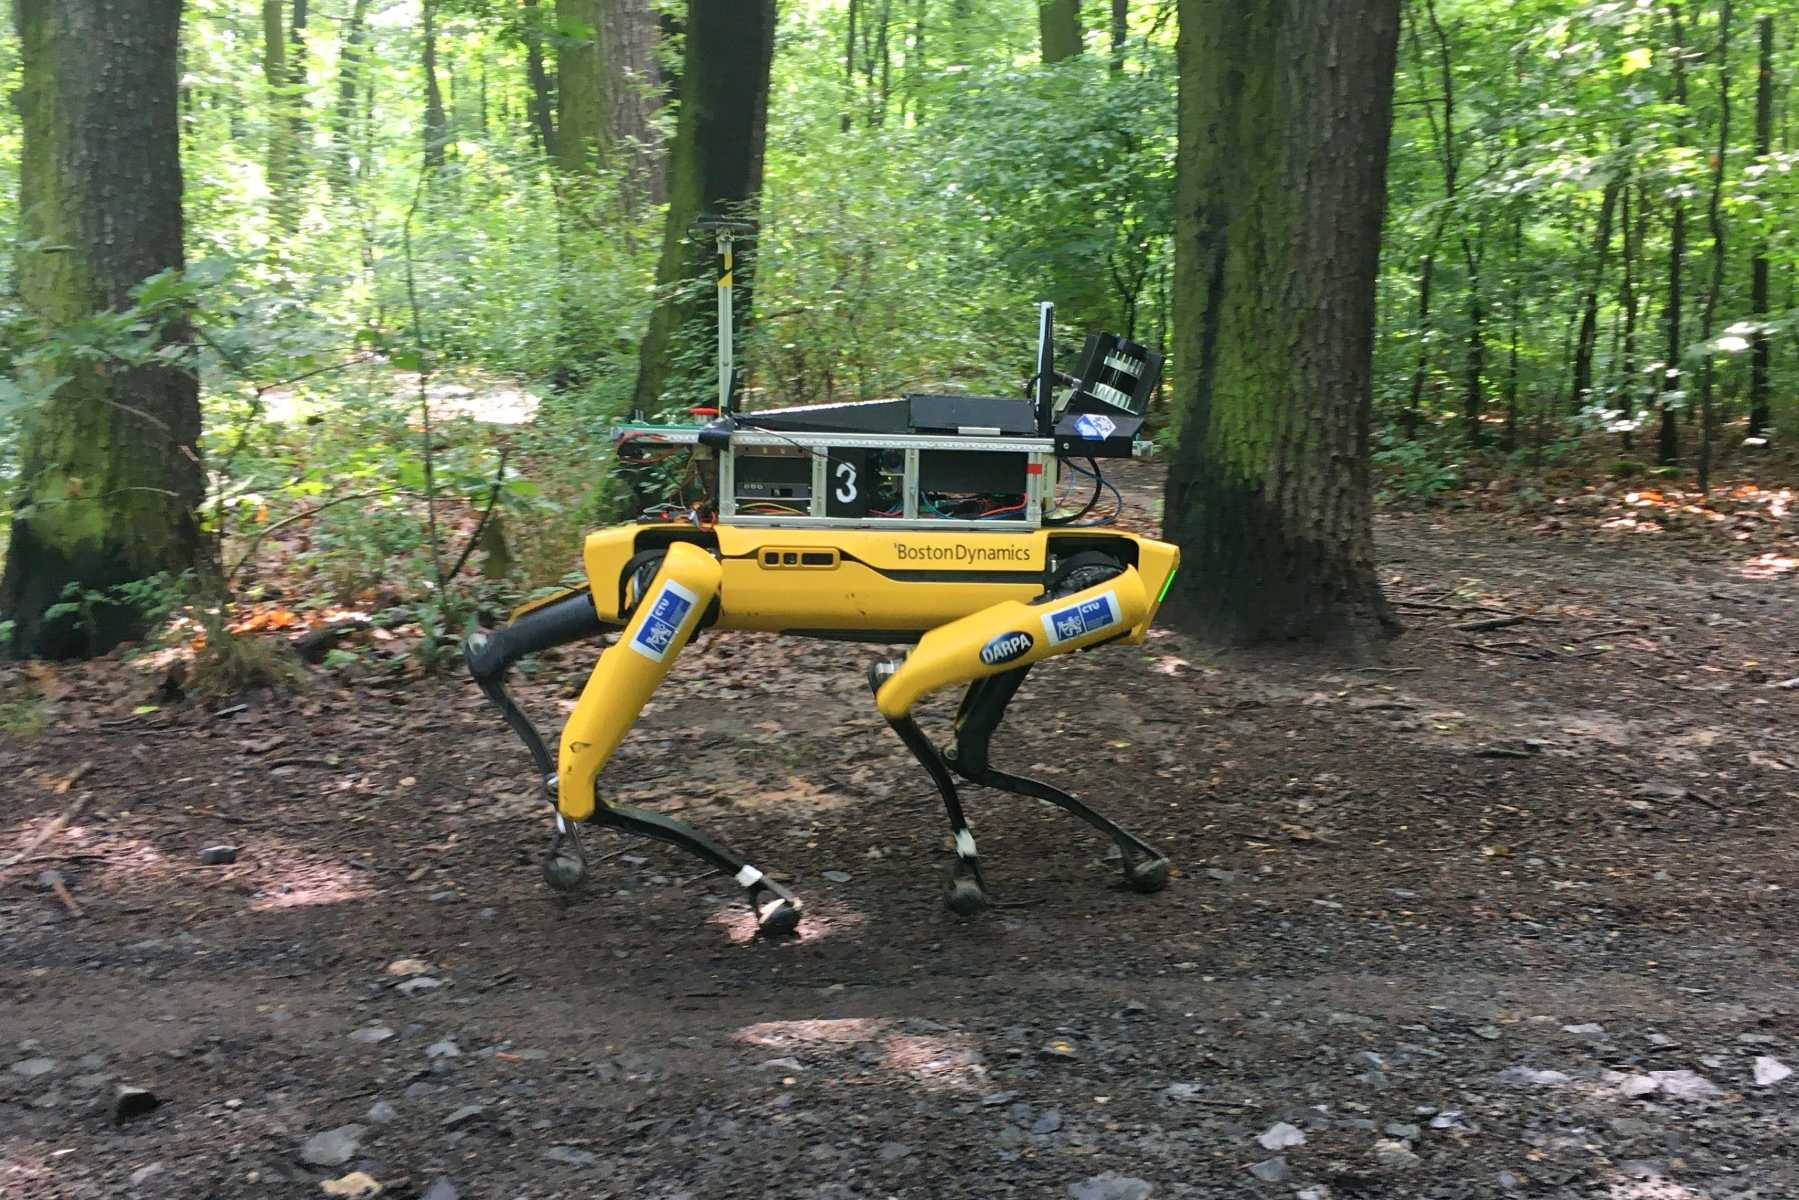
\includegraphics[width=\textwidth]{images/spot.jpg}
                \caption{The Spot robot configuration.}
                \label{fig:spot}
            \end{subfigure}
            \caption{Robots used in the real-world experiments.}
        \end{figure}
        \noindent The photos are courtesy of CRAS at FEE CTU.

    \subsection{Sensors}
        The capabilities of our robots are highly dependent on the sensors we attach to them. Without them, the possibilities and options for missions are minimal. In our work, we will use some sensors directly and some indirectly. The indirect usage of sensors is connected with dependencies on other projects. One notable example is the detection of vehicles and other obstacles. This detection is not in the scope of our work but is instrumental to its success.\\\\
        \bfc{Magnetometer}\\
            This is one of the sensors we use directly. We use it to determine the azimuth of our robot and help it position itself perpendicular to the road it will try to cross.\\
            We say that the sensor is used directly. However, the transformation of the IMU magnetometer data into the azimuth was not implemented as a part of this work.\\\\
        \bfc{Camera}\\
            Our robots are fitted with cameras pointing forward, backward, left, right, and up. This sensor is mostly used to determine the classification of obstacles rather than detecting the obstacles themselves. As this sensor is not vital to the functionality of our algorithm, we will not discuss them further.\\
            The cameras on our robots are GigE Basler ace2 PRO.\\\\
        \bfc{LiDAR}\\
            LiDAR is another essential sensor installed on our robots. It is responsible for detecting approaching vehicles and providing information such as their speed, position vectors, and other relevant parameters. The data generated by LiDAR plays a critical role in our algorithm, serving as the primary condition for switching between different modes of crossing.\\
            More detailed information on the scanning mechanisms and function of LiDARs can be found in \cite{LiDAR}.\\
            The LiDARs used on our robots are Ouster OS0-128.\\\\
        \bfc{GNSS}\\
            All robots also have a GPS sensor. We use this sensor for precise localization of the robots in the global coordinate system.\\
            The GPS sensors we use are Emlid Reach M+.

        \section{Simulation environment}
    For the simulation environment, we will use the Gazebo simulator. This simulator has direct support for ROS. We also have models of the Husky robot we can use to evaluate the behaviour of our algorithm.        

    \chapter{Behavior tree algorithm structure}

    \chapter{Nodes implementation}
        This chapter will provide the implementation details for individual nodes used in our BT algorithm. We will split these descriptions into BT nodes, and auxiliary functions used in the nodes.
        This chapter will provide the implementation details for individual nodes used in our BT algorithm. We will split these descriptions into BT nodes and auxiliary functions used in the nodes. We will also provide the implementation details for ROS nodes and other ROS-related parts.

\section{Behavior tree nodes}
    Here we will present the implementation of individual nodes in our algorithm. We will split the nodes into categories based on the sub-tree they belong to. We will also show the basic functionality of the library used.
    \subsection{Introduction}
        The BT algorithm is implemented using the behaviortree-cpp-v3 library. Therefore, we will present how we create, implement and start polling the tree. We will also show how nodes are created, implemented, and used.\\\\
        \bfc{Creating the node}\\
            To create the node, we need to create a class that inherits from one of the parent classes in the library. The parent classes depend on the type of node we want to create. If we create an action node, we inherit from the \texttt{SyncActionNode} class. If we create a condition node, we will inherit from the \texttt{ConditionNode} class.\\
            There are two mandatory functions for all nodes, the \texttt{tick} and \texttt{providedPorts} functions. These two functions must be implemented, or an error will occur.\\
            The \texttt{tick} function is responsible for the actual implementation of the node. It is called every time the node is ticked. It is also responsible for returning the state of the node.\\
            The \texttt{providedPorts} function defines the ports the node will use. This function must be defined even if the node does not use any ports.\\\\
        \bfc{Using the node}\\
            To use a node, we must register it in the \texttt{BehaviorTreeFactory} object. We do this by calling the \texttt{registerNodeType} function. For this function, we need to specify the class of the node we want to register, e.g., one of the nodes we created. It also takes one \texttt{std::string} parameter, which identifies the name of the node in our BT algorithm \texttt{.xml} file.\\\\
        \bfc{Creating and running the tree}\\
            To create the tree, we first must have a \texttt{.xml} file with the tree structure. This file is then parsed by the \texttt{BehaviorTreeFactory} object using the \texttt{createTreeFromFile} function. The result is a \texttt{Tree} object which we can store and later run. Ahead of calling the parsing for the tree file, all the nodes used in the file must be registered.\\
            To run the tree, we call the \texttt{tickRoot} function on the \texttt{Tree} object. This function returns the state of the root node of the tree.\\\\
        \bfc{Blackboard}\\
            The blackboard is a shared memory between the nodes of the tree. It is used to store data that is being utilized by multiple nodes.\\
            It is also the reason why we implement the \texttt{providedPorts} function. This function specifies the ports the node will use. The ports can serve as an \texttt{input}, an \texttt{output}, or both. \texttt{Input} ports can take a constant value (specified in the \texttt{.xml} file of the tree structure) or look for a value in the blackboard.\\\\
        \bfc{Logging}\\
            The BT library also provides us with logging functionality. This functionality is useful for debugging and testing.\\
            We can use different types of loggers. The most common one is the \texttt{StdCoutLogger} which logs to the standard output. We can also use the \texttt{FileLogger}, which saves logs to a file.\\
            We will use the \texttt{FileLogger} to log the tree execution. This logger is useful for its integration with the \texttt{Groot} application as we can import the produced file and visualize the ticking of our BT structure.\\
            The logging will be used only for debugging and testing purposes and serves no other function in the final product.
    \subsection{Main BT}
        In this BT, we only have one non-sub-tree node. This is because this sub-tree encodes the algorithm's structure rather than having nodes for execution.\\\\
        \bfc{StartAlgorithm -- Condition node}\\
            This node is responsible for determining whether the robot is in the phase of crossing the road during its mission. It is necessary to implement such a node to facilitate the transfer of control from path planning to road crossing. In contrast, we could determine if the crossing should start based on the distance of the robot from the road. However, this method would fail whenever our robot has to walk alongside any road.\\
            This node is implemented as a ROS service updating a static variable, which is checked when the node is ticked.\\
            This service should be used mainly by other nodes outside of the package itself, with one notable exception. The exception being the very last node of our tree. It serves as a prevention against the looping of our algorithm.
    \subsection{Init BT}
\label{sec:Init-BT-impl}
    Here we will present the nodes used in the Init sub-tree. This sub-tree is used to initialize the BT algorithm. It is the first sub-tree to be executed. This tree is going to be executed only once per road crossing.\\\\
    \bfc{GetPosition -- Action node}\\
        This node is responsible for obtaining the current GPS position of the robot and converting it to the UTM coordinate system. It is implemented as a ROS topic subscriber. The topic subscribed is \texttt{/gps/fix} where the GPS data are being published.\\
        The obtained data are then converted to UTM using the \texttt{gps\_to\_utm} function defined in \ref{sec:geo_func}. The result is then stored as two BT blackboard variables -- \texttt{easting} and \texttt{northing}.\\
        For every obtained value, it also calls a ROS service \texttt{place\_suitability} to determine the suitability of the current position for crossing.\\\\
    \bfc{CrossRoad -- Condition node}\\
        This node tells our algorithm if we are close enough to a road to take over the robot's controls. If we are not the path-planning or other node is left in control.\\
        We use the return values of the ROS service call issued in the \texttt{GetPosition} node. This service has two return values -- \texttt{validity} and \texttt{suitability}. \texttt{Suitability} uses the road cost as well as context score to judge the place for crossing. For \texttt{validity}, we only calculate the distance of the current location to road segments from OSM.\\
        Therefore the \texttt{validity} variable is the one determining the output of this node. The distance limit we proposed as sufficient is $10\:\rm{m}$ from the center of the road.\\\\
    \bfc{PlaceSuitable -- Condition node}\\
        This node states whether the current robot's location, stored as a blackboard variable, is suitable for crossing.\\
        It uses the second return value from the ROS service called in the \texttt{GetPosition} node. As stated, this value takes into account the road cost for our location from the road-cost algorithm (\ref{sec:road_cost}) and the context score calculated separately before the service call.\\
        The context score is based on the contextual information that is available to us. This information may be passed from other nodes (e.g., computer vision node for detecting road parameters) or set by the operator.\\
        The calculation of the context score and the process of obtaining the contextual information is described in \ref{sec:context}.\\\\

    \noindent Other nodes shown it the BT structure (fig \ref{fig:Init-BT}) are currently returning \texttt{FAILURE}. These nodes are there to show the potential for further work. Their main purpose is to steer the robot to a more optimal location for crossing. In this work, we assume that the correct location was chosen in the pre-mission planning.
    \subsection{Perpendicular BT}
\label{sec:Perpendicular-BT-impl}
    The task of this tree is to position the robot perpendicular to the road. It is the second sub-tree to be executed, and as well as Init BT, it is used to prepare the robot for the crossing and is only executed once.\\\\
    \bfc{GetAzimuth -- action node}\\
        This node is responsible for obtaining the robot's current azimuth. We have a ROS subscriber listening to topic published by \texttt{compass} node\footnote{\url{https://github.com/ctu-vras/compass}}.\\
        The compass node may publish the azimuth in several different formats. In our program, we use the ENU format in radians. But if the compass node publishes the azimuth in a different format, we have subscribers that can convert it to the desired format.\\
        The azimuth is then stored as a blackboard variable \texttt{azimuth}.\\\\
    \bfc{RoadHeading -- action node}\\
        This node calculates the heading of the closest road to the robot. We take the current robot's position from the blackboard variable \texttt{easting} and \texttt{northing} and send a request to the ROS service \texttt{get\_road\_heading}.\\
        The service returns the two coordinate points representing the closest road segment's starting and ending points.\\
        We then calculate the heading of the road segment using the function defined in section \ref{sec:geo_func}.\\
        The calculated road heading is then stored as a blackboard variable \texttt{road\_heading}.\\\\
    \bfc{ComputeHeading -- action node}\\
        This node uses the blackboard variable \texttt{azimuth} and \texttt{road\_heading} to calculate the heading the robot should achieve to be perpendicular to the road.\\
        The calculation is defined in section \ref{sec:geo_func}.\\
        The result is stored as a blackboard variable \texttt{req\_azimuth}.\\\\
    \bfc{RobotPerpendicular -- condition node}\\
        This node checks if the robot is perpendicular to the road. It works by comparing the current azimuth with the required heading. Both of these values are stored in the blackboard.\\
        We use the function defined in section \ref{sec:math_func} to compare the values to calculate the difference between two angles. The result is then compared to the threshold value, which is set to $0.1745\:\rm{rad}$ or $10\rm{^{\circ}}$.\\\\
    \bfc{RotateRobot -- action node}\\
        This node rotates the robot to the required heading.\\
        First, we calculate the difference between the robot's current and desired azimuth. Then, based on the difference, we proportionally set the rotation direction and speed.\\
        The calculated movement is then published to the \texttt{cmd\_vel} topic.\\\\
    \bfc{StepFromRoad -- action node}\\
        If, for whatever reason, the robot is not able to rotate safely, primarily due to the possibility of ending on the road, we use this node to move the robot away from the road.\\
        Firstly we check the difference between the robot's current azimuth and the road heading. Based on the difference, we set the direction of the movement.\\
        The movement is then published to the \texttt{cmd\_vel} topic.

    \subsection{Crossing BT}
\label{sec:Crossing-BT-impl}
    This tree is used for the main decision-making process. It is the third sub-tree to be executed, and the only one to be executed repeatedly.\\
    In multiple nodes we will use information about the detected vehicles, and collision parameters for each vehicle. Therefore, we first need to define the data structures used to store this information.\\\\
    \bfc{Vehicle data}\\
        The data structure for storing the information about the detected vehicles is defined as follows:
        \begin{lstlisting}[language=C++, caption={Vehicle data structure}, label={lst:vehicle_data}]
            struct vehicle_info {
                int id;
                double x_pos;
                double y_pos;
                double x_dot;
                double y_dot;
                double x_ddot;
                double y_ddot;
                double length;
                double width;
            };
            struct vehicles_data {
                int num_vehicles;
                std::vector<vehicle_info> data;
            };
        \end{lstlisting}
        The first struct \texttt{vehicle\_info} is used to store the information about single detected vehicle. The position of the vehicle is expressed in relation to the robot's frame. The robot frame means, the center of the robot is the origin of the coordinate system. The $x$-axis points forward from robot and the $y$-axis points to the left.\\
        The second struct \texttt{vehicles\_data} is used to store the \texttt{vehicle\_info} structs of all detected vehicles.\\\\
    \bfc{Collision data}\\
        The data structure for storing the collision parameters has the following definition:
        \begin{lstlisting}[language=C++, caption={Collision data structure}, label={lst:collision_data}]
            struct collision_info {
                int car_id;
                double v_front;
                double v_back;
                bool collide;
                bool collide_stop;
            };
            struct collisions_data {
                int num_collisions;
                std::vector<collision_info> data;
            };
        \end{lstlisting}
        The first struct \texttt{collision\_data} is used to store the collision parameters for single vehicle.\\
        The \texttt{v\_front} and \texttt{v\_back} variables are the velocities of the robot to come into contact with the front or back of the vehicle. The figure \ref{fig:collision} shows the contact points we are calculating the velocities for. The figure is explained in the next part.\\
        The \texttt{collide} variable is a boolean value that tells us if the robot is going to collide with the vehicle. It is calculated based on the current velocities of the robot and the vehicle.\\
        The second struct \texttt{collisions\_data} is used to store the information about collisions with all detected vehicles.\\\\
    \bfc{Used units}\\
        We use these units for the measured and calculated parameters:
        \begin{itemize}
            \item \textbf{Position} -- meters $[\rm{m}]$
            \item \textbf{Time} -- seconds $[\rm{s}]$
            \item \textbf{Velocity} -- meters per second $[\rm{m\,s^{-1}}]$
            \item \textbf{Acceleration} -- meters per second squared $[\rm{m\,s^{-2}}]$
            \item \textbf{Dimensions} -- meters $[\rm{m}]$
        \end{itemize}
    \bfc{Calculating the collision parameters}\\
        First, we need to state the assumptions we are making in order to simplify the calculation.\\
        The first assumption is about the coordinate system we are using. We are using the robot's frame, where the robot's center is the system's origin, and all the positions are expressed in relation to this origin. The $x$-axis points forward, and the $y$-axis points to the left. We can assume this because the calculations are done periodically, and the results are only relevant for the current time step. It also simplifies the process, as the vehicle positions are already expressed in the robot frame.\\
        The second assumption is about the movement of the robot. We assume the robot is moving in a straight line with constant velocity. This is reasonable as we want the robot to be as predictable as possible, so we do not want to move the robot to the side. The assumption about the constant velocity, meaning the acceleration is zero, is also reasonable. The speeds the robot can achieve are much lower than the robot's acceleration, we can therefore neglect the acceleration.\\
        The third assumption is about the movement of the vehicle. We assume the vehicle's acceleration is constant. This is a reasonable simplification as the calculation is done periodically.\\
        The fourth assumption is that we will calculate the collision only in two dimensions. This is reasonable as the $z$-axis will not impact the occurance of a collision. Moreover, the area over which the collision can occur is relatively small, and therefore, any terrain deviation will not impact the collision significantly.\\\\
        Figure \ref{fig:collision} depicts a schematic view of the collision. There are two contact points, both on the robot and the vehicle. The first one (blue) is the point where the robot is going to collide with the front of the vehicle. The second one (red) is the point where the robot is going to collide with the back of the vehicle.\\
        \begin{figure}[ht]
            \centering
            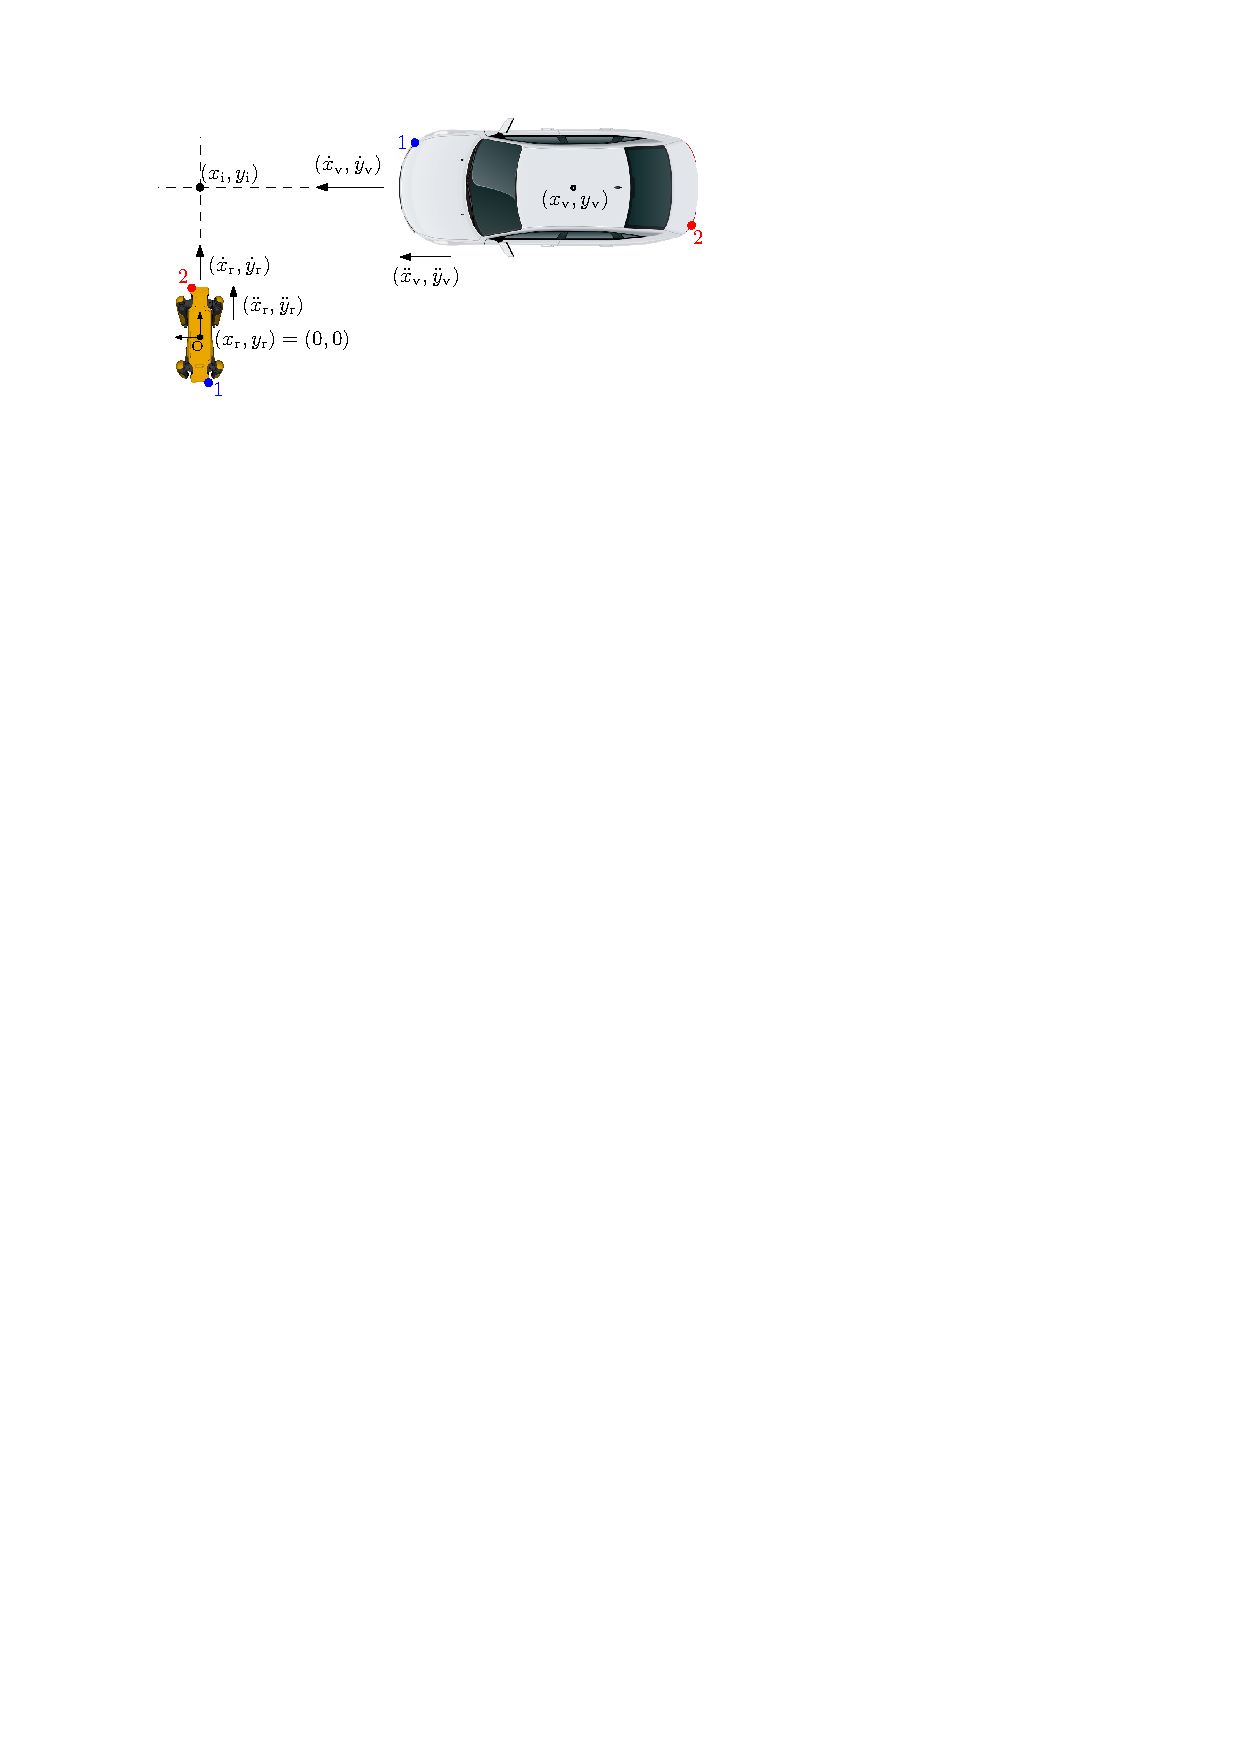
\includegraphics[height=6cm]{images/collision.pdf}
            \caption{Visualization of collision points, coordinate system, and vehicle parameters.}
            \label{fig:collision}
        \end{figure}
        \noindent For the first point, we calculate the velocity \texttt{v\_front}. This velocity depicts the minimal speed of the robot to cross in front of the vehicle. We calculate the velocity \texttt{v\_back} for the second point. This velocity depicts the maximal speed of the robot to cross behind the vehicle.\\
        The subscript \texttt{r} is used for parameters of the robot, and the subscript \texttt{v} is used for parameters of the vehicle.\\
        The calculation is divided into three parts. In the first part, we determine the starting positions of the robot and the vehicle. In the second part, we calculate the time when the vehicle will reach the intersection point $(x_{\rm{i}}, y_{\rm{i}})$. In the last part, we calculate the velocities for the robot to collide with the vehicle.\\\\
        The first part is necessary as the coordinates of both the robot and the vehicle are at the center of their respective bodies. We need to move the starting points concerning the robot's and vehicle's length and width. The starting points for the robot are calculated using these equations:
        \begin{align}
            x_{\rm{r,f}} &= \frac{l_{\rm{r}}+w_{\rm{v}}}{2},\\
            x_{\rm{r,b}} &= -\frac{l_{\rm{r}}+w_{\rm{v}}}{2},\\
            y_{\rm{r,f}} &= y_{\rm{r,b}} = 0,
        \end{align}
        where $l_{\rm{r}}$ is the length of the robot and $w_{\rm{v}}$ is the width of the vehicle.\\
        The starting points for the vehicle are calculated as follows:
        \begin{align}
            x_{\rm{v,f}} &= x_{\rm{v}} + \frac{l_{\rm{v}}+w_{\rm{r}}}{2}\cos{(\varphi_{\rm{v}})},\\
            x_{\rm{v,b}} &= x_{\rm{v}} - \frac{l_{\rm{v}}+w_{\rm{r}}}{2}\cos{(\varphi_{\rm{v}})},\\
            y_{\rm{v,f}} &= y_{\rm{v}} + \frac{l_{\rm{v}}+w_{\rm{r}}}{2}\sin{(\varphi_{\rm{v}})},\\
            y_{\rm{v,b}} &= y_{\rm{v}} - \frac{l_{\rm{v}}+w_{\rm{r}}}{2}\sin{(\varphi_{\rm{v}})},
        \end{align}
        where $\varphi_{\rm{v}} = \arctan{\left(\frac{\dot{y}_{\rm{v}}}{\dot{x}_{\rm{v}}}\right)}$ is the angle of the vehicle, $l_{\rm{v}}$ is the length of the vehicle and $w_{\rm{r}}$ is the width of the robot.\\
        We put the width of the robot to the calculation of the vehicle's starting points and vice versa because we want to flatten the dimensions of the objects. This is done to simplify the calculation of the intersection point of the robot's and vehicle's trajectory.\\
        The second part of the calculation is further divided into two parts. The reason is, that there are two possible scenarios for the calculation. We will use the general equation of motion \cite{equation_motion} for both calculations.\\
        In the first scenario, the vehicle's acceleration in the $y$-axis is zero. That means we can calculate the time using the following equations:
        \begin{align}
            t_{\rm{f}} = -\frac{y_{\rm{v,f}}}{\dot{y}_{\rm{v}}},\\
            t_{\rm{b}} = -\frac{y_{\rm{v,b}}}{\dot{y}_{\rm{v}}}.
        \end{align}
        In the second scenario, the acceleration of the vehicle in the $y$-axis is non-zero. This scenario is more probable, as vehicles rarely drive at a constant speed. In this case, the time is calculated in the following way:
        \begin{align}
            t_{\rm{f},1,2} = \frac{-\dot{y}_{\rm{v}}\pm\sqrt{\dot{y}_{\rm{v}}^2-2\ddot{y}_{\rm{v}}y_{\rm{v,f}}}}{\ddot{y}_{\rm{v}}},\\
            t_{\rm{b},1,2} = \frac{-\dot{y}_{\rm{v}}\pm\sqrt{\dot{y}_{\rm{v}}^2-2\ddot{y}_{\rm{v}}y_{\rm{v,b}}}}{\ddot{y}_{\rm{v}}}
        \end{align}
        There are two possible solutions for each time. The reason is that the vehicle may be decelerating and therefore change the direction of its travel. The interpretation of the results and the selection of the correct solution is discussed in the next section.\\
        The last part of the calculation is the calculation of the velocities. First, we need to calculate the position of the vehicle in the $x$-axis at the time of the collision. We use the general equation of motion with $t_{0}=0\:\rm{s}$:
        \begin{align}
            x_{\rm{i,f}} &= x_{\rm{v,f}} + \dot{x}_{\rm{v}}t_{\rm{f}} + \frac{1}{2}\ddot{x}_{\rm{v}}t_{\rm{f}}^2,\\
            x_{\rm{i,b}} &= x_{\rm{v,b}} + \dot{x}_{\rm{v}}t_{\rm{b}} + \frac{1}{2}\ddot{x}_{\rm{v}}t_{\rm{b}}^2.
        \end{align}
        Now we can calculate the velocities of the robot.
        \begin{align}
            \dot{x}_{\rm{r,f}} &= \frac{x_{\rm{i,f}}-x_{\rm{r,b}}}{t_{\rm{f}}},\\
            \dot{x}_{\rm{r,b}} &= \frac{x_{\rm{i,b}}-x_{\rm{r,f}}}{t_{\rm{b}}}.
        \end{align}
        The calculated velocities may be positive or negative. The interpretation is explained in the following section.\\\\
    \bfc{Interpretation of the calculated collision parameters}\\
        We will divide this section into two parts. The first part is the interpretation of the calculated time. The second part is the interpretation of the calculated velocities.\\\\
        If the calculated time is positive, the intersection point of the robot's and vehicle's trajectory is in the future. This means that the robot can collide with the vehicle without either of them changing the direction of travel.\\
        If the calculated time is negative, it means that the intersection point of the robot's and vehicle's trajectory is in the past. This means that the robot can collide with the vehicle, but only if the vehicle or the robot changes the direction of travel.\\
        The time can also be zero. This means that the robot and vehicle already collided. Therefore, we do not expect such time to arise as a result of the calculation.\\
        We may have up to two solutions when calculating the times for non-zero acceleration. If we have none, the robot's and the vehicle's trajectories do not intersect.\\
        If we have one solution, the robot's and the vehicle's trajectories intersect only once. The interpretation is that the vehicle is decelerating and will stop at the intersection point and then start reversing.\\
        If we have two solutions, the robot's and the vehicle's trajectories intersect two times. Multiple intersections could have several physical interpretations. We can interpret this as the vehicle decelerating, and therefore, changing the direction of travel after passing the intersection point. We can also interpret this as the vehicle accelerating, and therefore, the second time of the intersection is likely negative.\\
        When choosing the calculated time, we will use the following criteria. If one time is positive and the second is negative, we will use the positive time. If both times are positive, we will use the shorter time. If both times are negative, we will use the larger time (the time that is closer to the present).\\\\
        The velocities can also be positive or negative. The interpretation is similar to the one of time. Positive velocity means moving forward, while negative velocity means moving backward.\\
        While it may seem irrelevant to calculate the time and velocity for backward movement, it is essential. The reason is that some other vehicle may be moving so that the robot would collide with it. In that case, the robot will have to move backward to avoid the collision, and we need to be able to set the correct backward velocity to not collide with the first vehicle.\\\\
    \bfc{GetCars -- action node}

    
        \section{Auxiliary functions}
    In this section, we will present the auxiliary function used in the nodes of our BT algorithm.\\
    These will include the functions used for conversions, more complex or repetitive mathematical operations, and other functions that are not directly related to the BT algorithm.\\
    One of the big sections will be the algorithms used for determining the classification and cost of roads in the road network.\\
    We will split the functions into categories based on their purpose.

    \subsection{Road cost algorithm}
        \label{sec:road_cost}
        We will use the algorithm developed during the summer of 2022 for the RobInGas project at the CTU CRAS. The algorithm was designed to determine the cost of crossing the road based on the road classification, curvature, and other factors.\\
        We will briefly present the functionality of the algorithm. The full description with implementation details can be found in \cite{Road_cost_docs}.\\
        This is also the only part of our thesis written in Python instead of \CC\ this is due to it being part of a different project. Other reasons include the usage of libraries for Python. While we could rewrite the code to \CC\ it was not deemed necessary as this part is run only once at the beginning of the mission and therefore does not need to be optimized for speed.\\\\
        \bfc{Overview}\\
            We use multiple parameters to determine the cost of crossing. The most important ones are the geometrical properties of the road. This includes the curvature of the road, the elevation profile, and the proximity to intersections. We also use the road classification to add to the cost function.\\
            Other parameters would be beneficiary, such as the road width, the presence of a pedestrian crossing, and the expected traffic speed.\\
            Unfortunately, we do not have access to all of these parameters. We use the OSM data, which does not necessarily contain all those additional parameters. Therefore, we will inject this information directly into the algorithm and deal with these parameters separately.\\
            The OSM data also do not contain the elevation profile of the road. This data is also not easily obtainable from free or open-source sources. The elevation data we use were purchased from the Land Survey Office of the Czech Republic. We use the ZABAGED\footnote{\url{https://geoportal.cuzk.cz/(S(dcpfei0nmxcwgoe4frurwfgm))/Default.aspx?lng=EN&mode=TextMeta&text=dSady_zabaged&side=zabaged&menu=24}} data. This data from the Land Survey Office are available only for the area of the Czech Republic. However, any file with elevation data with the correct formatting can be used. The used file format is as follows. A text file with the easting, northing, and altitude of one point is on one line separated by a space. The lines are separated with a newline character \texttt{\textbackslash n}, each describing exactly one point.\\
            If the elevation data are not provided, the algorithm will still function. It will just not take the elevation profile into account. The road cost will be determined only from the curvate and road classification.\\\\
        \bfc{Algorithm}\\
            The algorithm is divided into several parts.\\
            The first part is obtaining the road segments from downloaded OSM data. This part is also responsible for logging the road classification for each segment.\\
            The second part is responsible for determining the curvature of the roads. This is done by calculating the radius of the circumcircle of the triangle formed by the two adjacent road segments. This approach is visualized in image \ref{fig:curvature}. We then sort the road segments into multiple classes based on their radius. In this part, we also detect road junctions and penalize the road segments close to the junction.\\
            In the third part, we determine the elevation profile of the road. We then classify the individual road segments with the TPI (Terrain Profile Index) method. Some TPI classes are presented in image \ref{fig:TPI}.\\
            In the last part, we combine the results from the previous parts and calculate the final cost of crossing for each segment.
            \begin{figure}[H]
            \centering
            \begin{subfigure}[b]{0.45\textwidth}
                \centering
                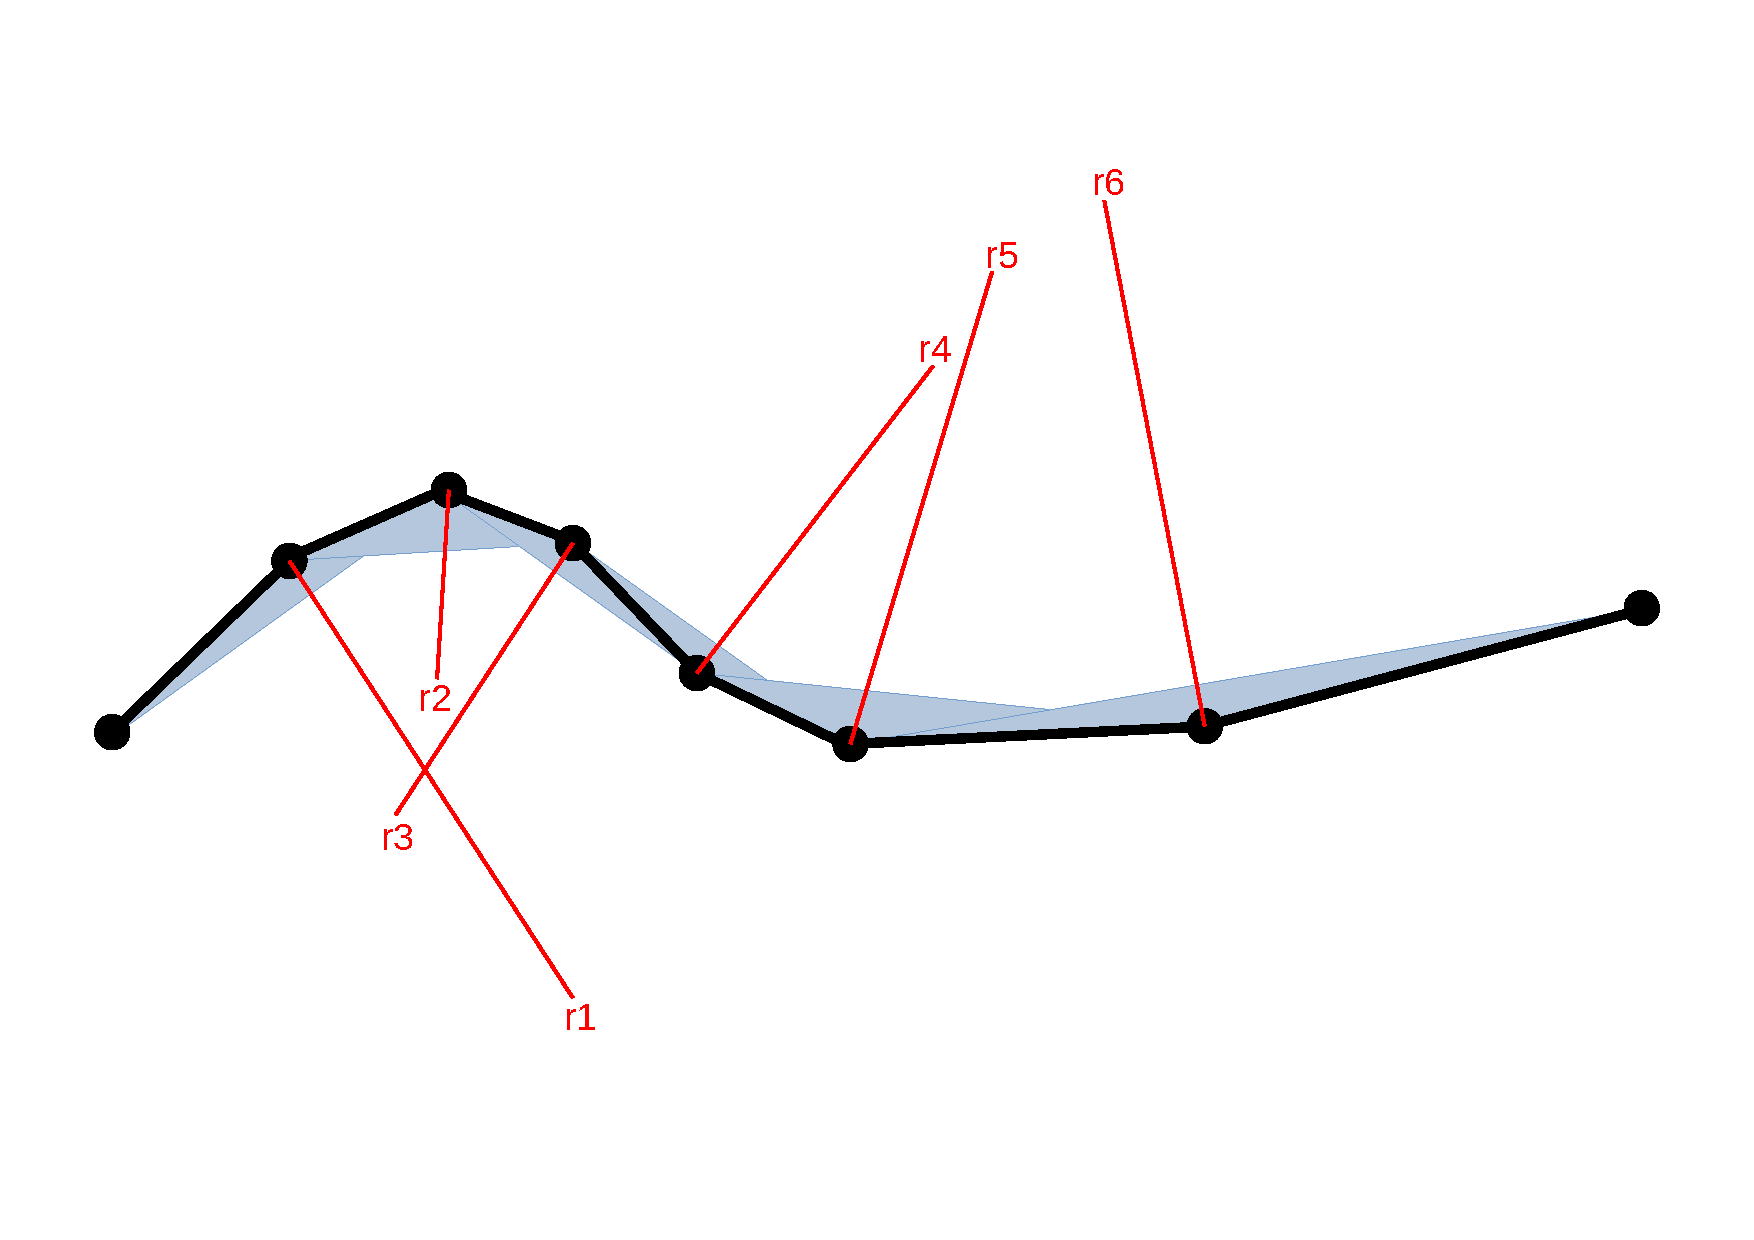
\includegraphics[width=\textwidth]{images/path_curvature.pdf}
                \caption{Visualization of the circumcircle radii.}
                \label{fig:curvature}
            \end{subfigure}
            \begin{subfigure}[b]{0.45\textwidth}
                \centering
                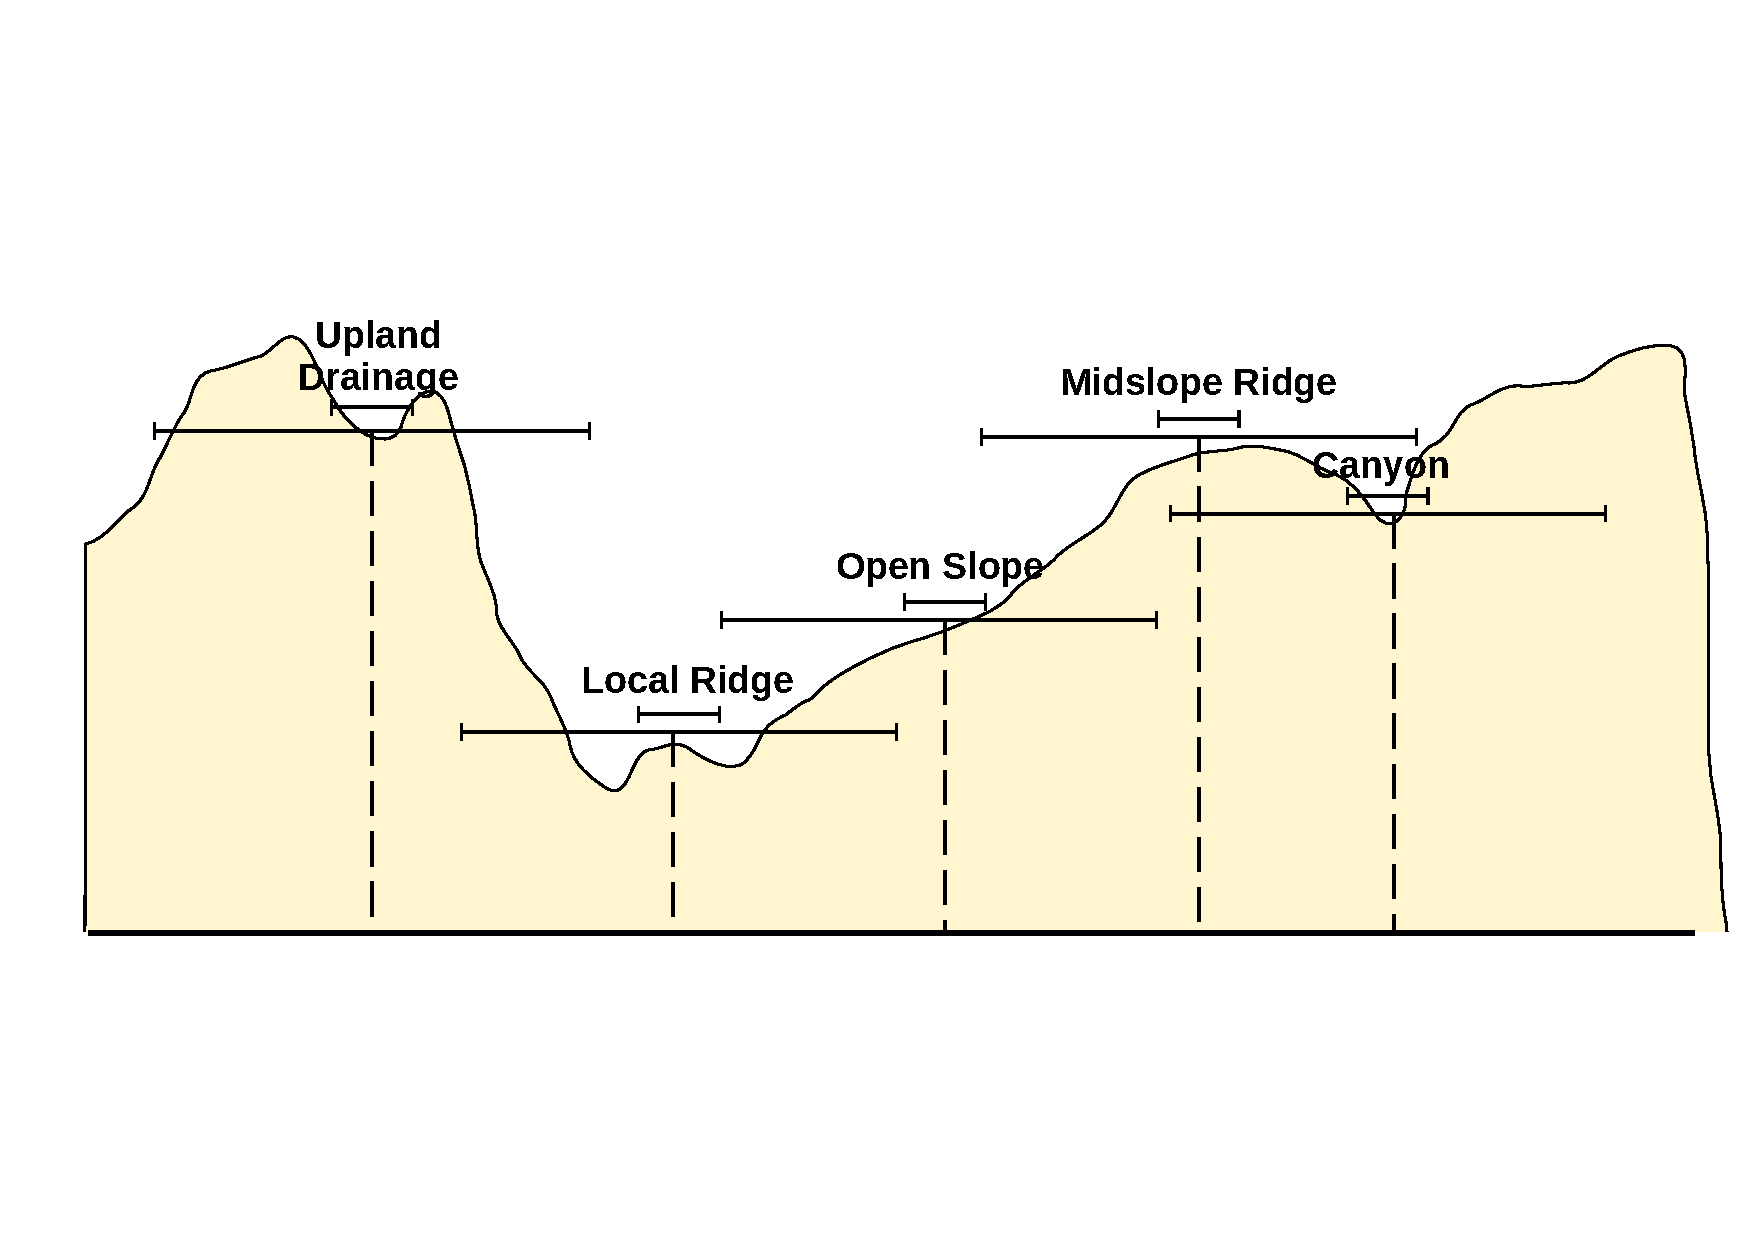
\includegraphics[width=\textwidth]{images/TPI_classification.pdf}
                \caption{Representation of certain TPI classes.}
                \label{fig:TPI}
            \end{subfigure}
            \caption{Visualization of key elements in road cost algorithm.}
        \end{figure}

        \bfc{Usage}\\
            As was stated earlier, this algorithm is executed only once at the beginning of the mission. Later we only keep the final costs, and based on them, we determine if the location where the robot is trying to cross is suitable and safe.\\
            We rely on ROS to enable the communication between our main algorithm and the algorithm for determining the suitability of the location for crossing. We use the ROS service for this purpose.\\
            Another part of the algorithm is to try and provide the robot with a more suitable place for crossing if the current location is unsuitable. If such a place is found and provided we will publish a cost map that will be used to change the current cost map of the path planner. This is done so that we do not need to override the robot's controls until we begin the crossing itself.

    \subsection{Mathematical functions}
        \bfc{Difference between two angles}\\
            This function is used to determine the difference between two given angles. We assume the angles given are in radians, and both are in the interval $\langle0;2\pi\rangle$. This difference is calculated to be the smallest possible and to fit within the interval $\langle-\pi;\pi\rangle$. The formula we use is a modified version of the one provided here \cite{calc_rotation}. The formula is as follows
            \begin{equation}
                \Delta\varphi = \left((\varphi_{2} - \varphi_{1} + \pi) \mod (2\pi)\right) - \pi.
            \end{equation}
            Before returning the result, we check whether the result is within the specified interval.\\\\
        \bfc{Converting degrees to radians}\\
            While this function is elementary in its nature, it is often used in our code. Therefore it is beneficiary to create this function.\\
            The equation for converting degrees to radians which this function uses, is as follows
            \begin{equation}
                \varphi_{\rm{RAD}} = \varphi_{\rm{DEG}}\:\frac{\pi}{180}.
            \end{equation}

    \subsection{Geographical functions}
    \label{sec:geo_func}
        Here we will present the functions used for geographical calculations. These include conversions between coordinate systems, calculating azimuths, and others.\\\\
        \bfc{Converting GPS to UTM}\\
            While most geographical data are stored in the WGS84 coordinate system, the UTM coordinate system is more suitable for calculations. We, therefore, need to convert the GPS coordinates to UTM.\\
            We use the GeographicLib library for this purpose. The function from this library that we use is \texttt{GeographicLib::UTMUPS::Forward}. This function takes the point's latitude and longitude and returns the point's easting and northing in the UTM coordinate system. It also returns the zone number and whether the point is in the northern or southern hemisphere.\\
            While the input variables are passed by value, the return variables are passed to the function call by reference.\\\\
        \bfc{Converting NED to ENU}\\
            There are two possible orientations of an azimuth. The NED (North-East-Down) and the ENU (East-North-Up).\\
            NED means that azimuth 0 points north, and its value increases clockwise. This orientation is mainly used in cartography and everyday life.\\
            ENU means that azimuth 0 points east, and its value increases clockwise. This orientation is mainly used in navigation and robotics, as it is consistent with REP-103.\\
            In the entire project, we use the ENU orientation. However, as we rely on other ROS nodes to provide us with the azimuth, we need to be able to convert the azimuth from NED to ENU.\\
            The conversion should be much simpler since we do not deal with coordinates but with already computed azimuths.\\
            The image \ref{fig:dir_indi} shows the two possible orientations of the azimuth. This image also provides us with the insight we need to determine the conversion formula. We need to divide the formula into two parts.
            \begin{figure}[H]
                \centering
                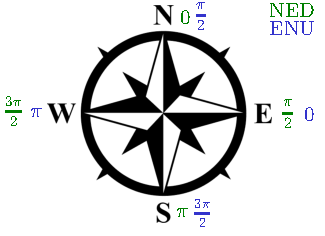
\includegraphics[width=0.5\textwidth]{images/direction_indicator.pdf}
                \caption{Two possible orientations of the azimuth.}
                \label{fig:dir_indi}
            \end{figure}
            \noindent The first option is when the azimuth (in NED) is between 0 and $\frac{\pi}{2}$ rad. In this case, the azimuth in ENU is computed in the following way
            \begin{equation}
                a_{\rm{ENU}} = \frac{\pi}{2} - a_{\rm{NED}},
            \end{equation}
            where $\text{a}_{\rm{ENU}}$ is the azimuth in ENU and $\text{a}_{\rm{NED}}$ is the azimuth in NED.\\
            The second option is for all other azimuths, e.g., when the azimuth is between $\frac{\pi}{2}$ and $2\pi$ rad. In this case, the azimuth in ENU is computed in the following way
            \begin{equation}
                a_{\rm{ENU}} = \frac{5\pi}{2} - a_{\rm{NED}}.
            \end{equation}\\\\
        \bfc{Compute azimuth from coordinates}\\
            This function is used to compute the azimuth for an observer standing at the first point and looking at the second point.\\
            We will use a slightly modified version of the formula provided here \cite{calc_bearing}. This calculation was created for the WGS84 coordinate system, however, we use the UTM coordinate system. Having said that, we can use the same formula, as the WGS84 to UTM projection is conformal\cite{Map_projections}.\\\\
        \bfc{Compute heading for robot}\\
            The use of this function is to determine the heading of the robot. It is used to get the robot perpendicular to the road.\\
            The function takes the robot's heading and the road's azimuth. The road azimuth was obtained using the function stated above.\\
            The algorithm creates two new variables, one $+\pi$ and one $-\pi$ from the road's azimuth. This is necessary as we do not know in what order are road points stored and we do not need to differentiate the side we approach the road from.\\
            Then it computes the difference between the robot's heading and the two new azimuths. The smallest difference is then returned.\\\\

        
    %\chapter{Simulation experiments}

    %\chapter{Real-world experiments}

    %\chapter{Discussion}

    %\chapter{Summary}

    \printbibliography

\end{document}